\documentclass[/home/jesse/Analysis/FemtoAnalysis/AnalysisNotes/AnalysisNoteJBuxton.tex]{subfiles}
\begin{document}

\subsection{Spherical Harmonics}
\label{AdditionalFigures_SphericalHarmonics}



\begin{figure}[h]
  \centering
  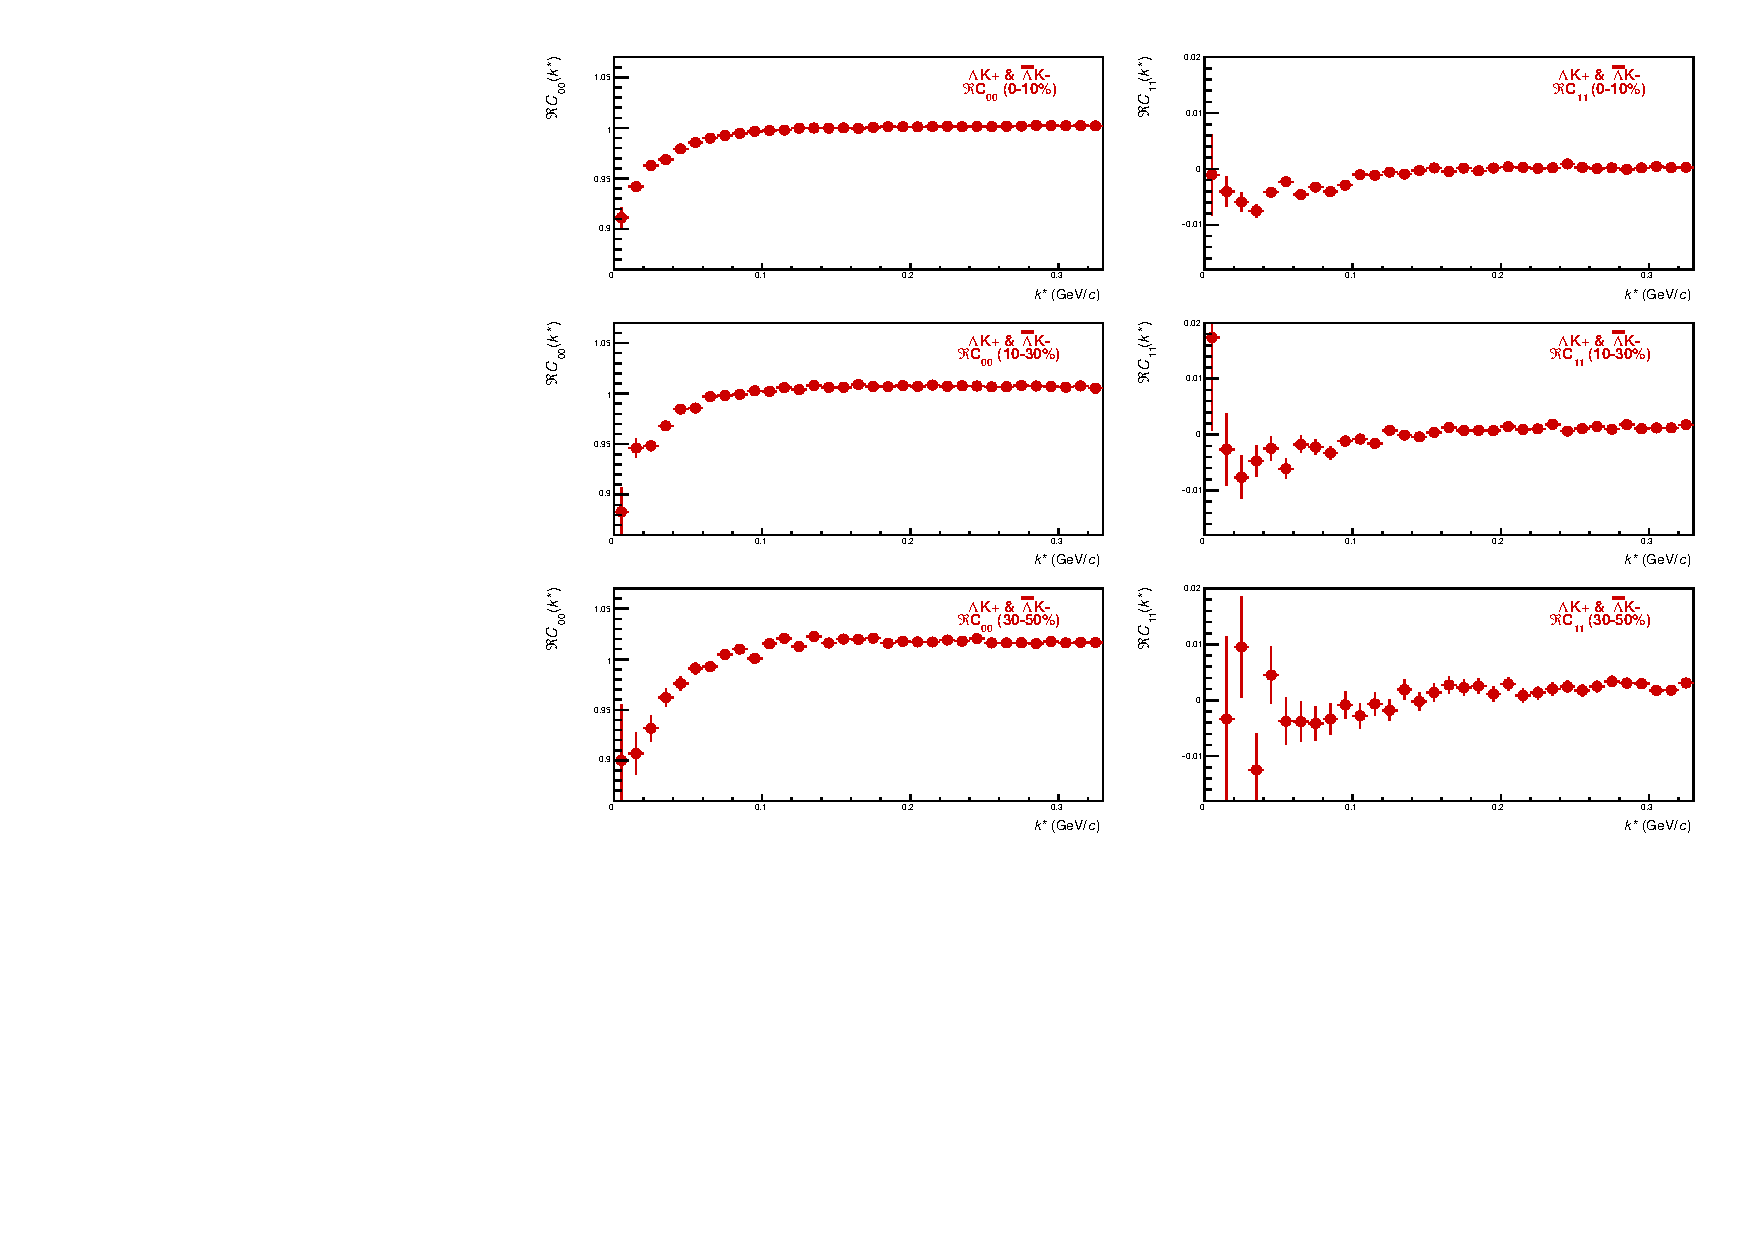
\includegraphics[width=\textwidth]{\ResultsDirBase Results_cLamcKch_20181205/SphericalHarmonics/LamKchP/CanCfYlmReC00C11_LamKchPALamKchM_All.pdf}
  \caption[Short Caption]{Long Caption}
  \label{fig:LamKchP_ReC00C11_All}
\end{figure}



\begin{figure}[h!]
  \centering
  %%----start of first subfigure---  
  \subfloat[Caption 1]{
    \label{fig:LamKchP_FirstSixCYlm:a}
    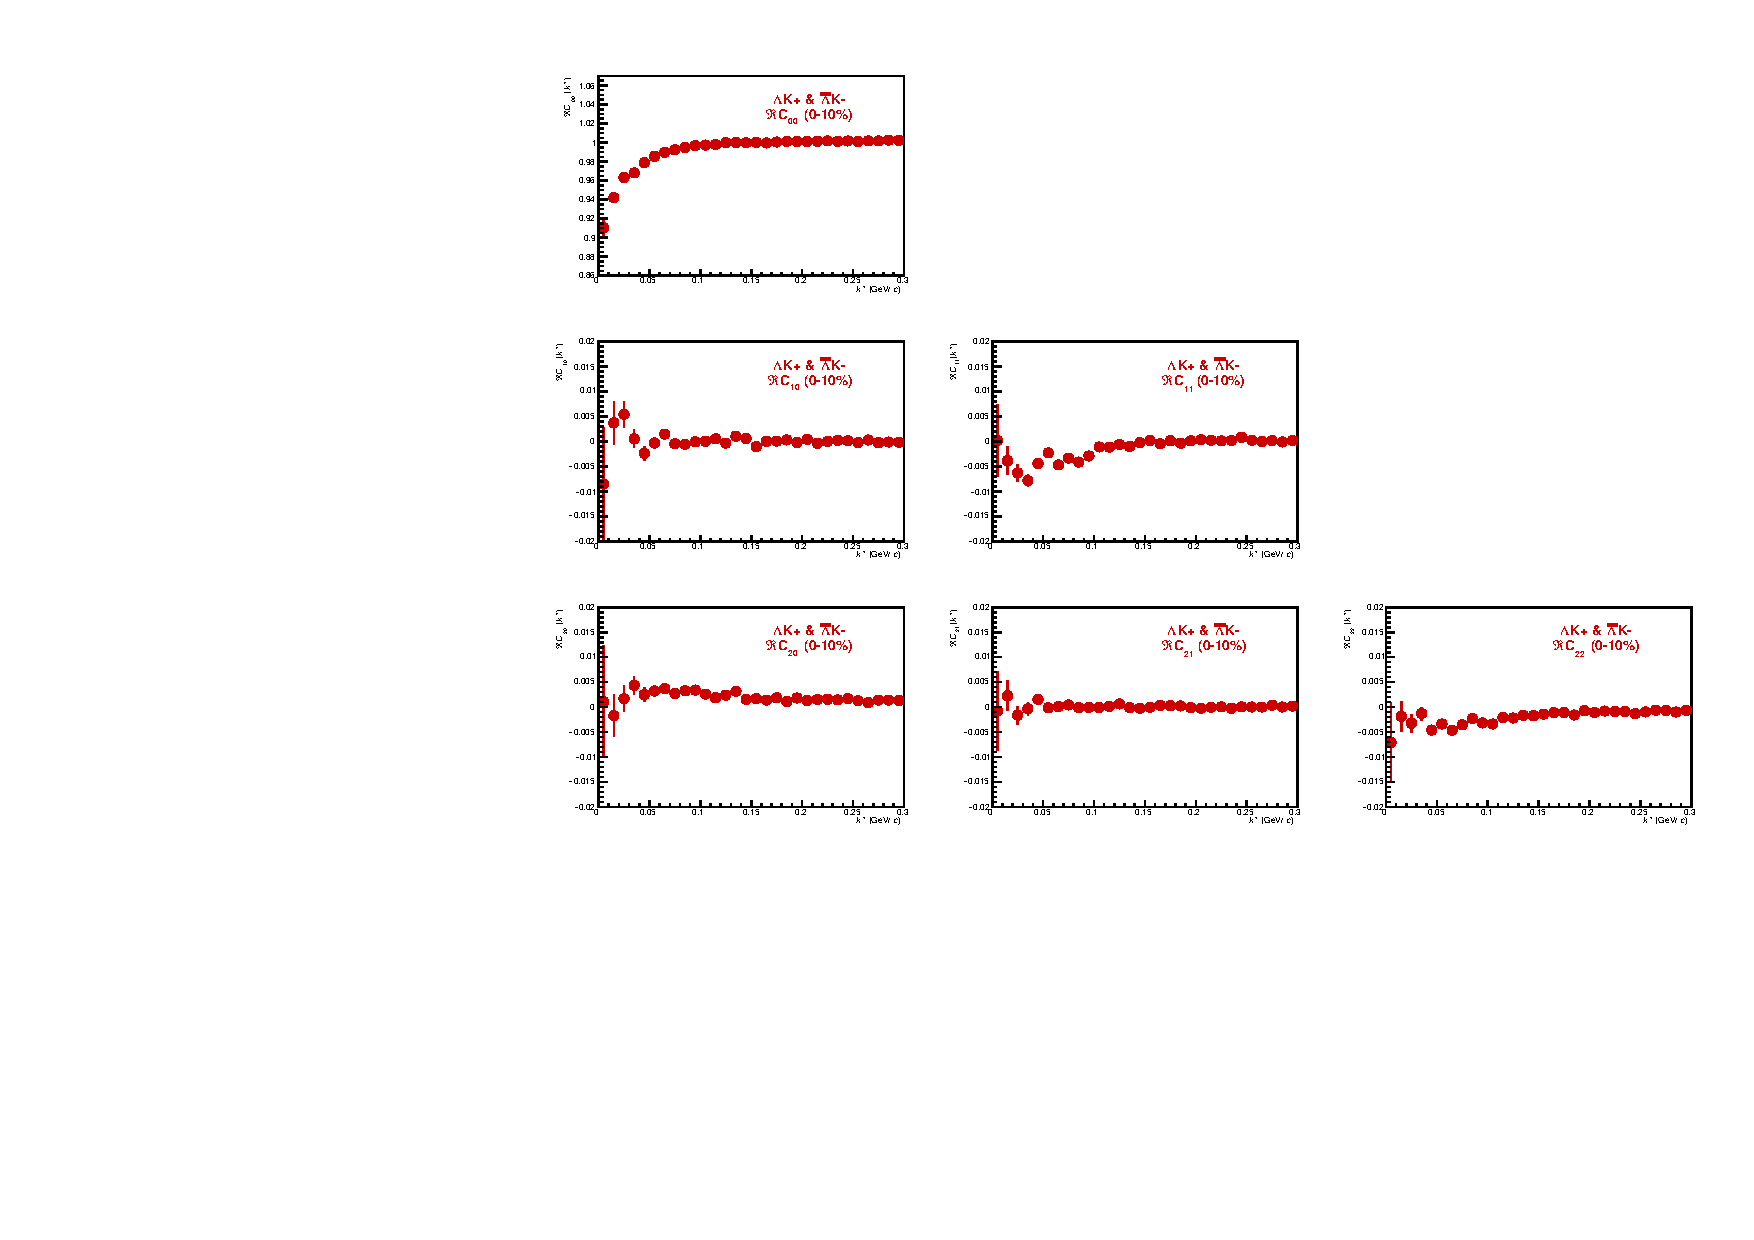
\includegraphics[width=0.50\linewidth]{\ResultsDirBase Results_cLamcKch_20181205/SphericalHarmonics/LamKchP/CanCfYlmReFirstSixComps_LamKchPALamKchM_0010.pdf}}
  %%----start of second subfigure---
  \subfloat[Caption 2]{
    \label{fig:LamKchP_FirstSixCYlm:b}
    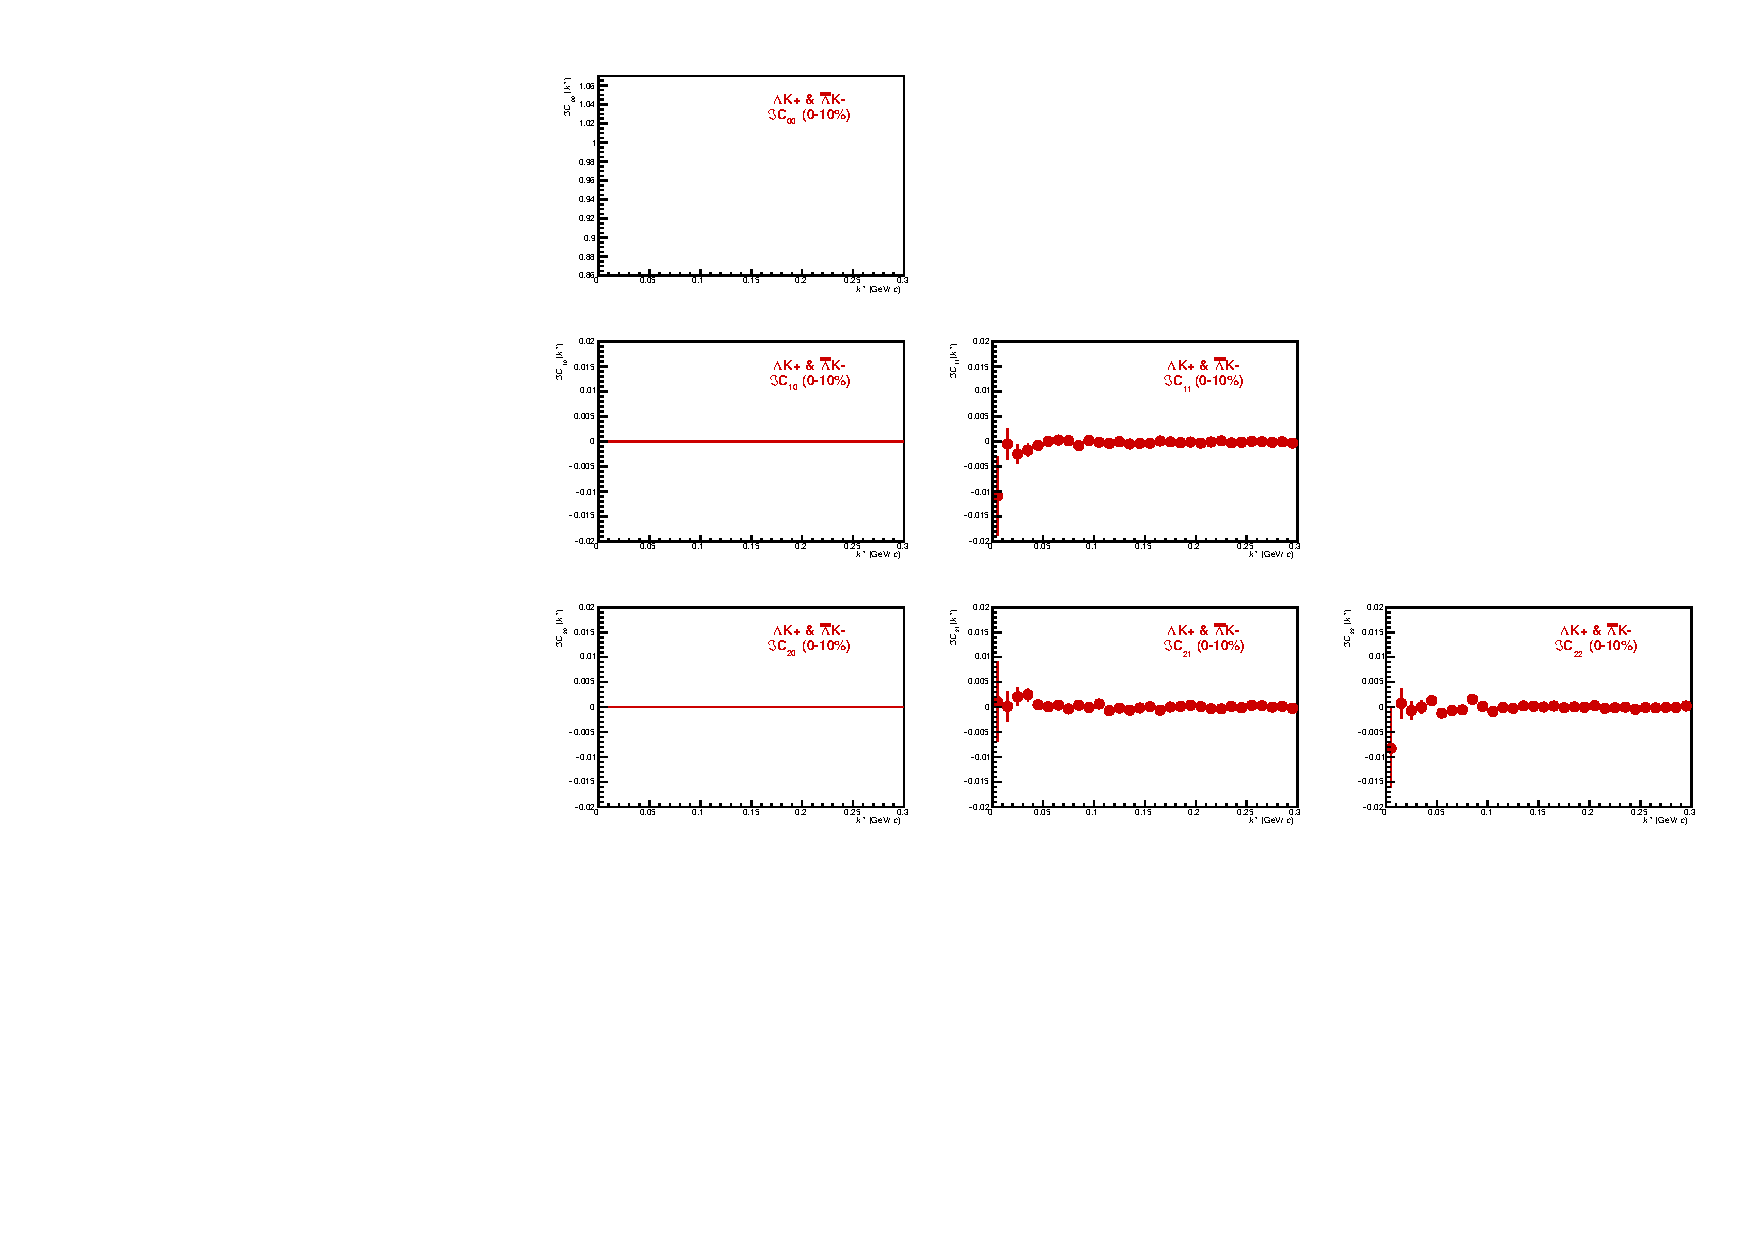
\includegraphics[width=0.50\linewidth]{\ResultsDirBase Results_cLamcKch_20181205/SphericalHarmonics/LamKchP/CanCfYlmImFirstSixComps_LamKchPALamKchM_0010.pdf}}  
  %%----overall caption----
  \caption[Short Overall]{Long Overall}
  \label{fig:LamKchP_FirstSixCYlm}
\end{figure}











\begin{figure}[h]
  \centering
  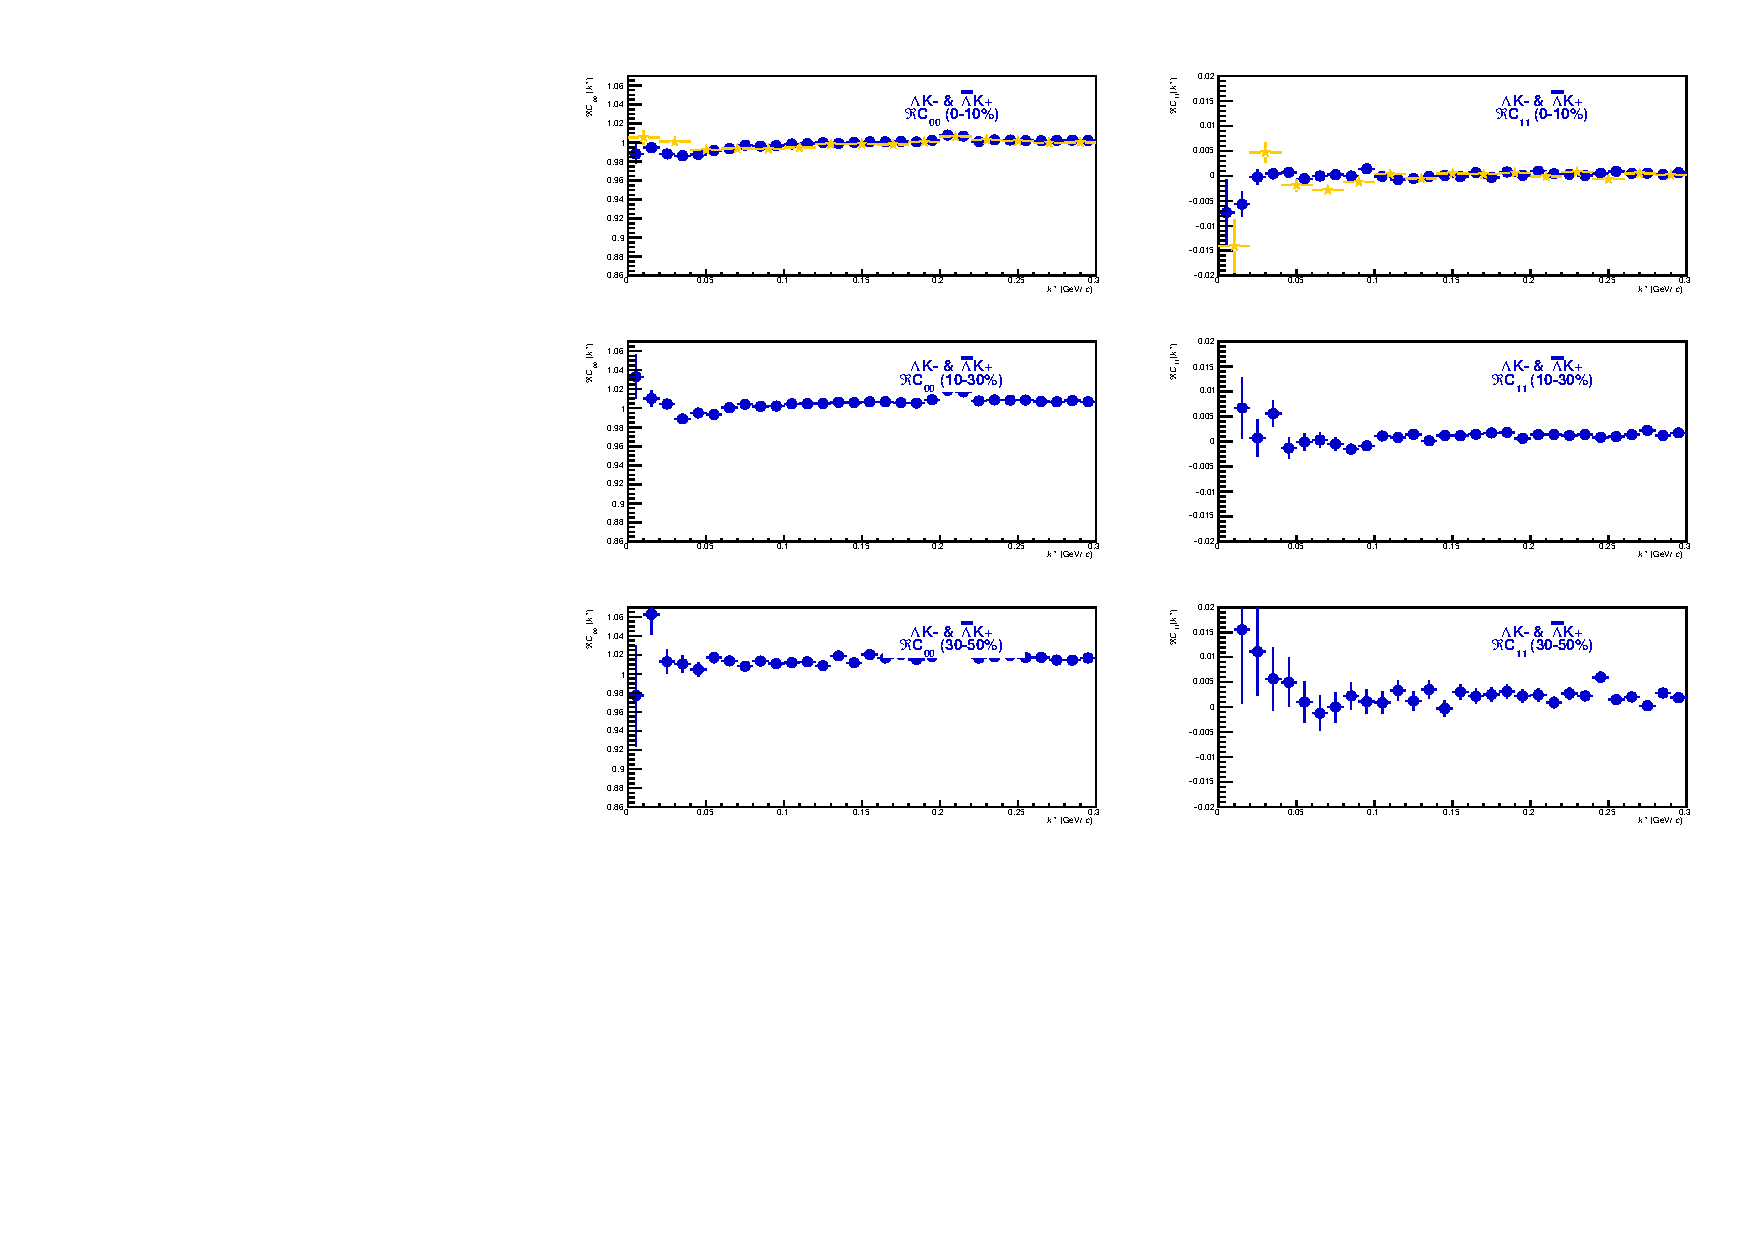
\includegraphics[width=\textwidth]{\ResultsDirBase Results_cLamcKch_20181205/SphericalHarmonics/LamKchM/CanCfYlmReC00C11_LamKchMALamKchP_All.pdf}
  \caption[Short Caption]{Long Caption}
  \label{fig:LamKchM_ReC00C11_All}
\end{figure}



\begin{figure}[h!]
  \centering
  %%----start of first subfigure---  
  \subfloat[Caption 1]{
    \label{fig:LamKchM_FirstSixCYlm:a}
    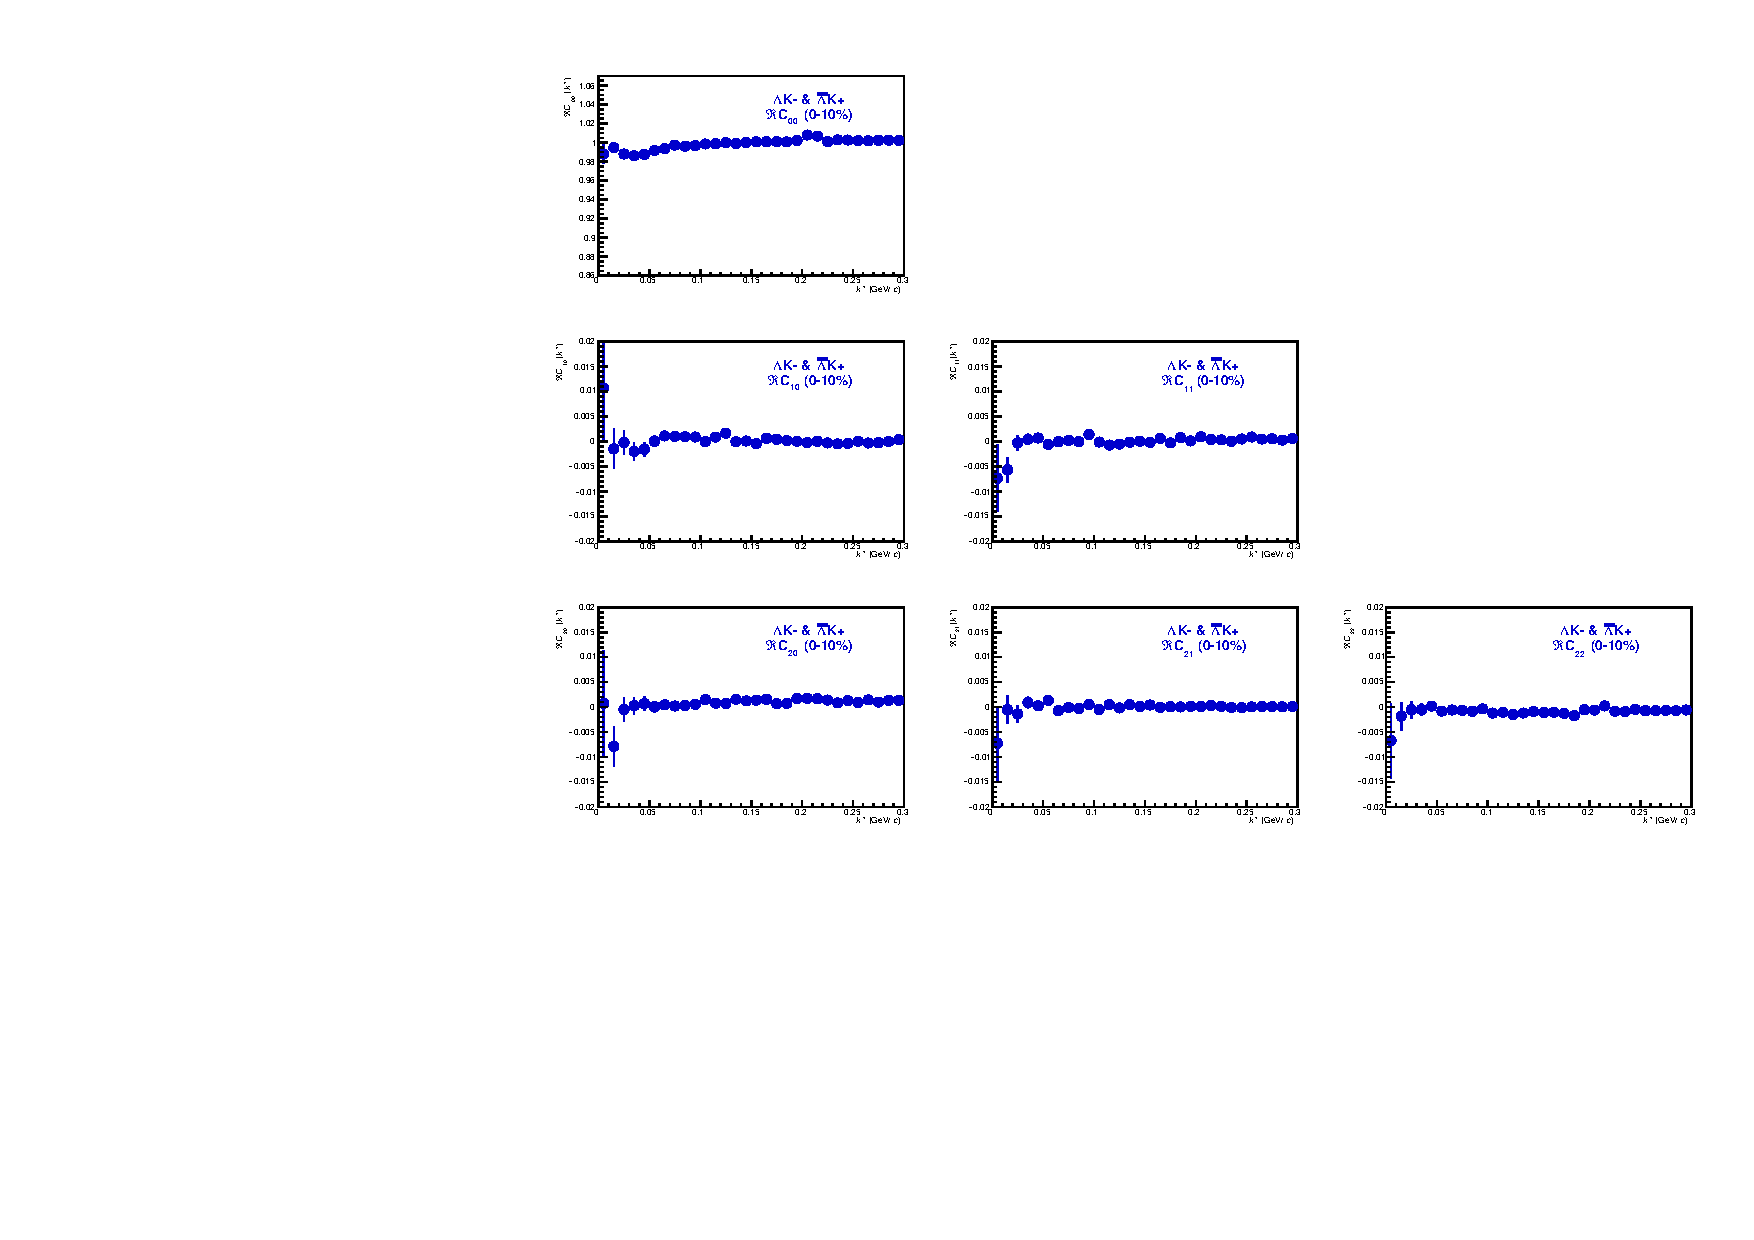
\includegraphics[width=0.50\linewidth]{\ResultsDirBase Results_cLamcKch_20181205/SphericalHarmonics/LamKchM/CanCfYlmReFirstSixComps_LamKchMALamKchP_0010.pdf}}
  %%----start of second subfigure---
  \subfloat[Caption 2]{
    \label{fig:LamKchM_FirstSixCYlm:b}
    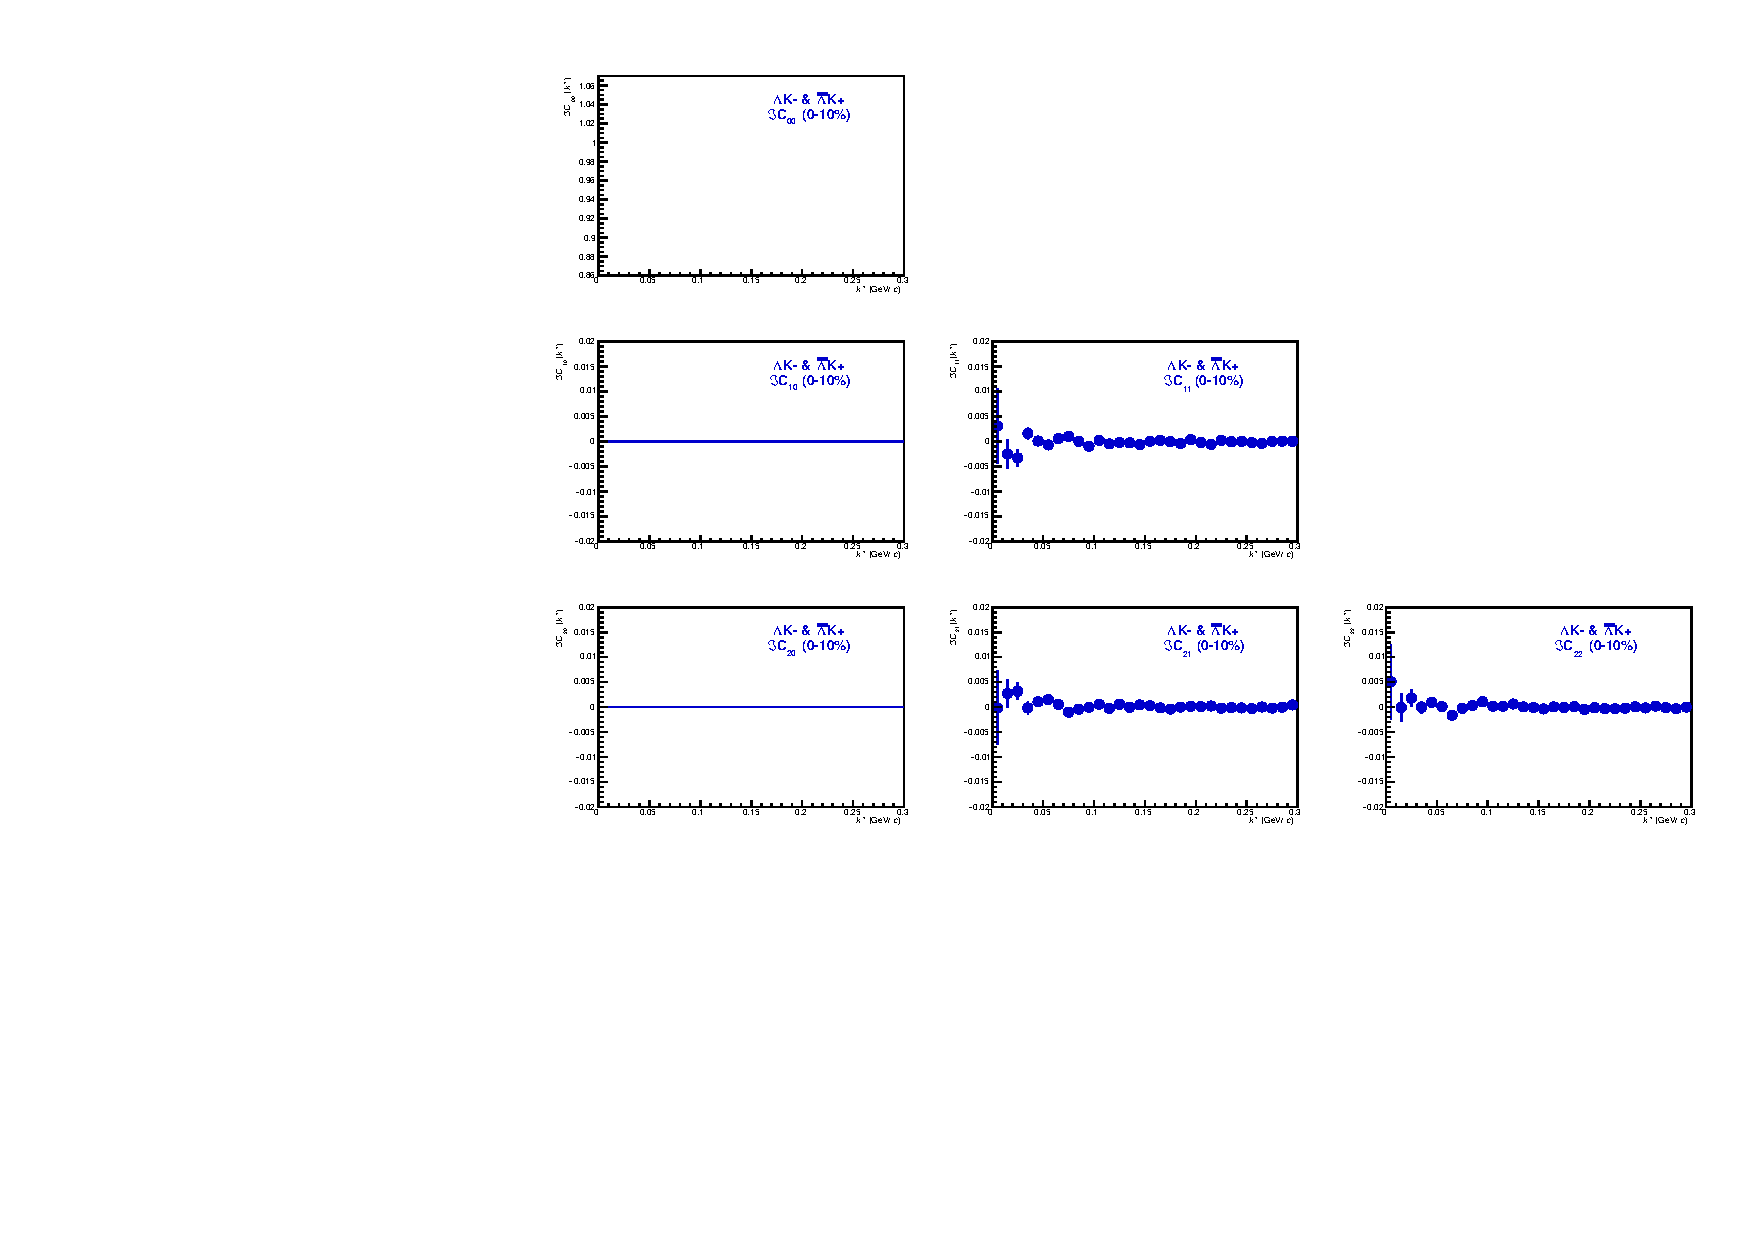
\includegraphics[width=0.50\linewidth]{\ResultsDirBase Results_cLamcKch_20181205/SphericalHarmonics/LamKchM/CanCfYlmImFirstSixComps_LamKchMALamKchP_0010.pdf}}  
  %%----overall caption----
  \caption[Short Overall]{Long Overall}
  \label{fig:LamKchM_FirstSixCYlm}
\end{figure}













\begin{figure}[h]
  \centering
  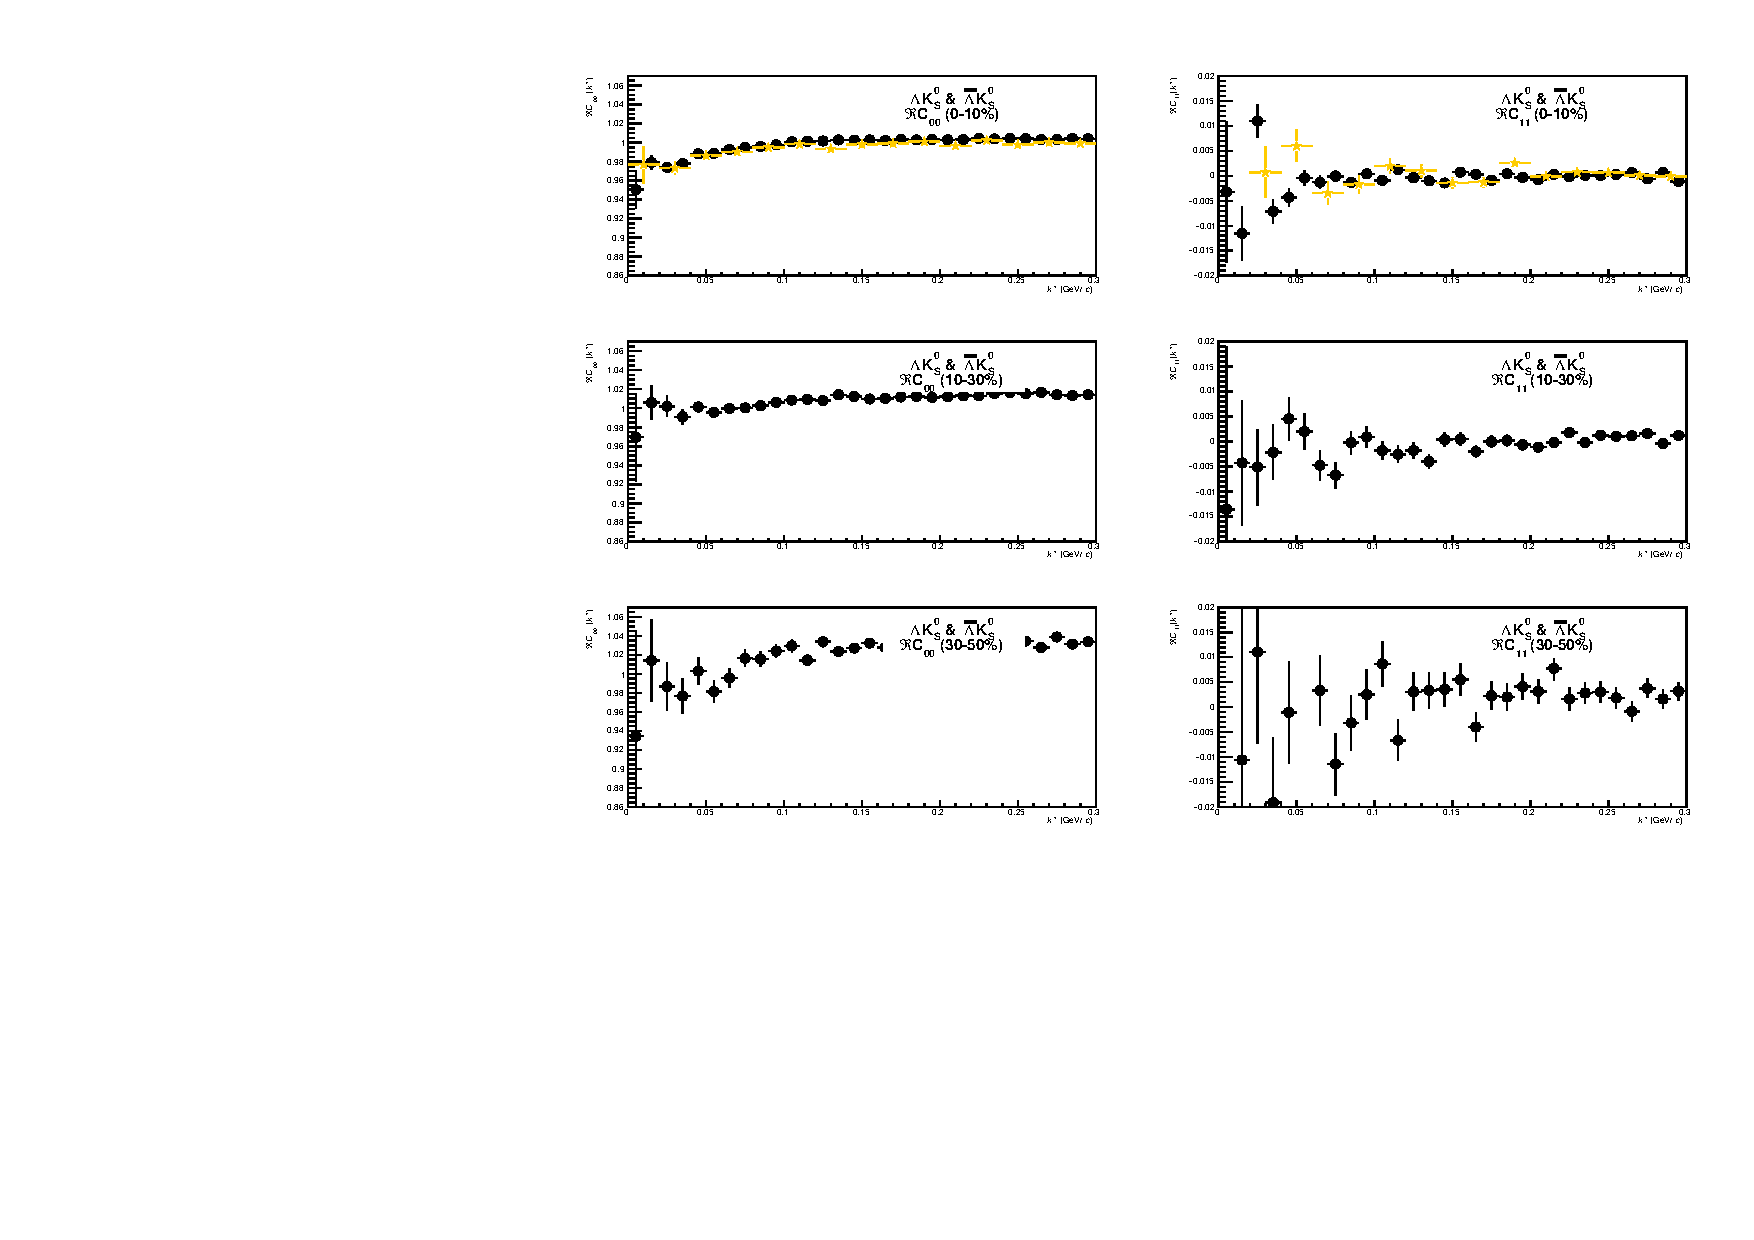
\includegraphics[width=\textwidth]{\ResultsDirBase Results_cLamK0_20181205/SphericalHarmonics/LamK0/CanCfYlmReC00C11_LamK0ALamK0_All.pdf}
  \caption[Short Caption]{Long Caption}
  \label{fig:LamK0_ReC00C11_All}
\end{figure}



\begin{figure}[h!]
  \centering
  %%----start of first subfigure---  
  \subfloat[Caption 1]{
    \label{fig:LamK0_FirstSixCYlm:a}
    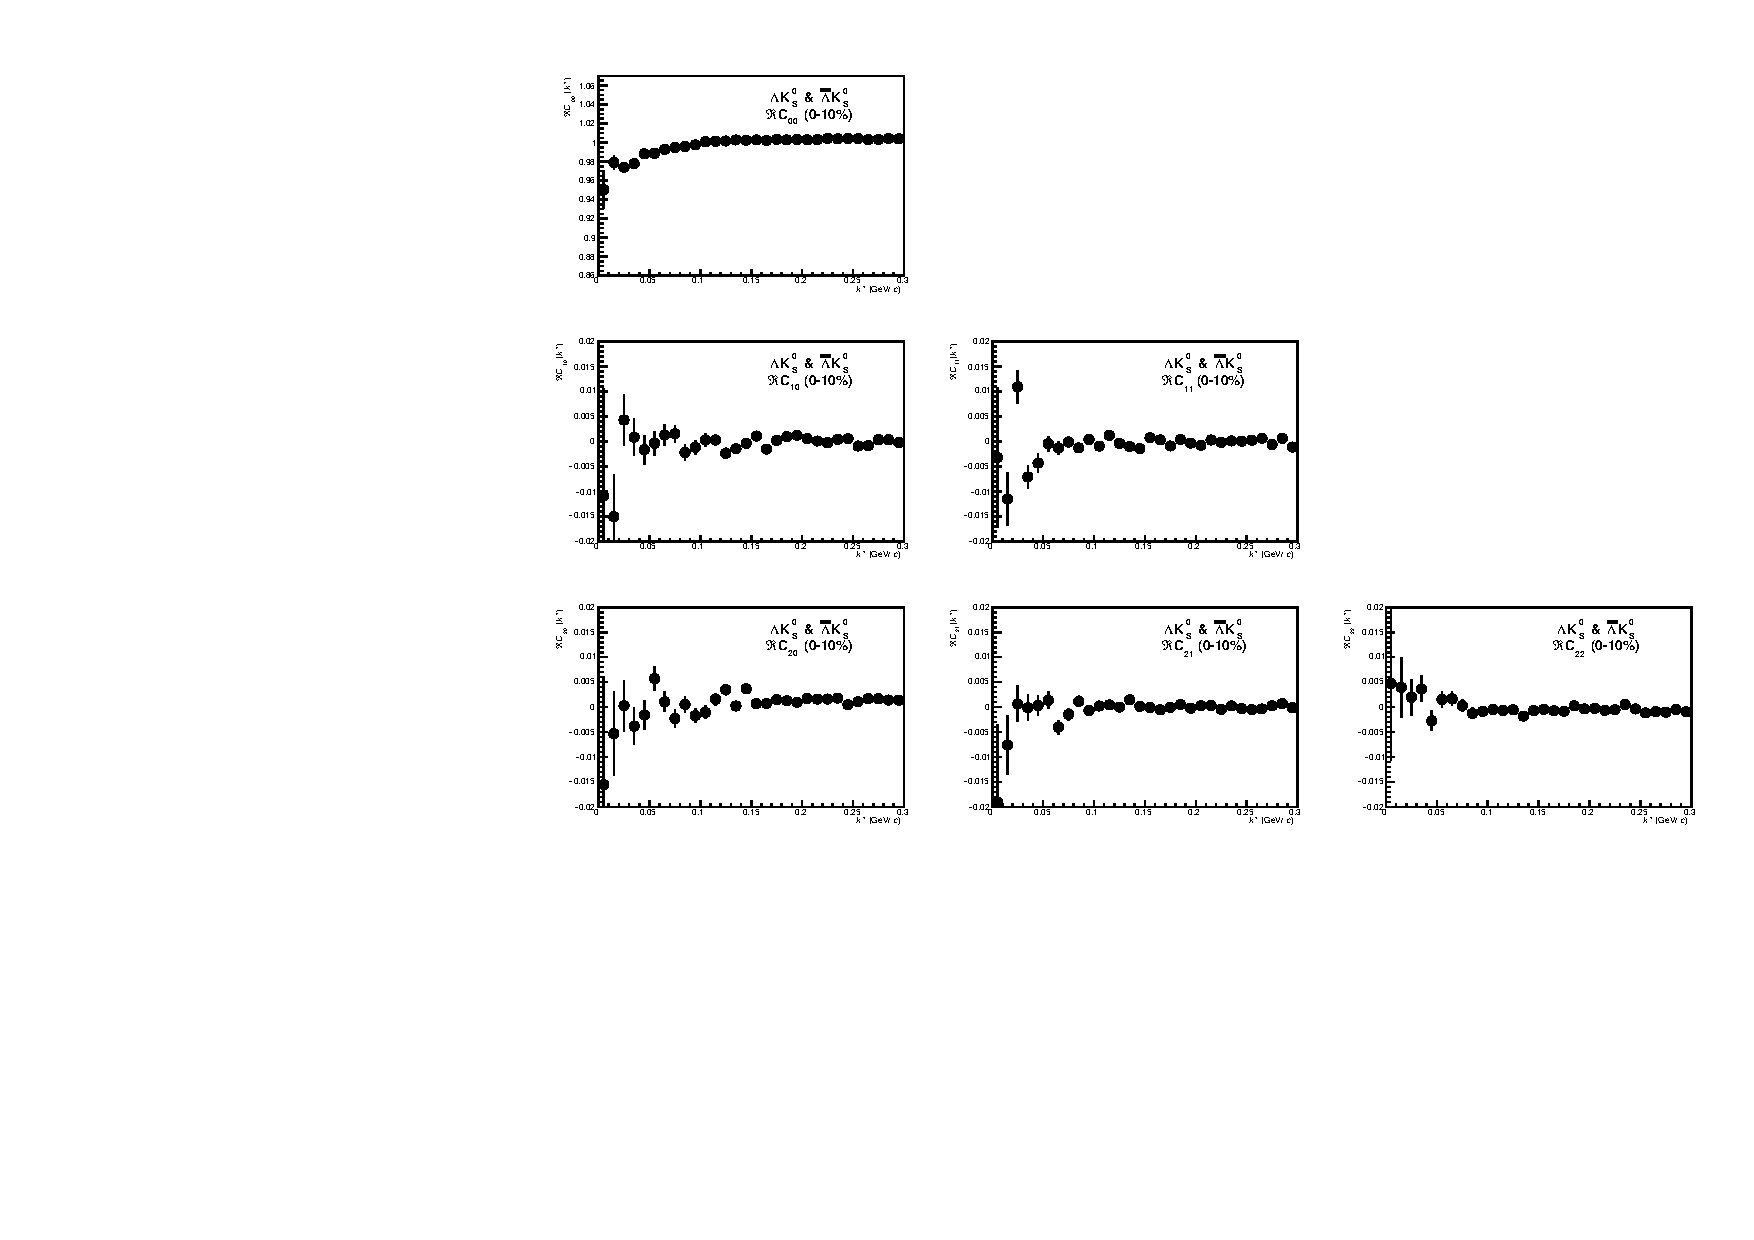
\includegraphics[width=0.50\linewidth]{\ResultsDirBase Results_cLamK0_20181205/SphericalHarmonics/LamK0/CanCfYlmReFirstSixComps_LamK0ALamK0_0010.pdf}}
  %%----start of second subfigure---
  \subfloat[Caption 2]{
    \label{fig:LamK0_FirstSixCYlm:b}
    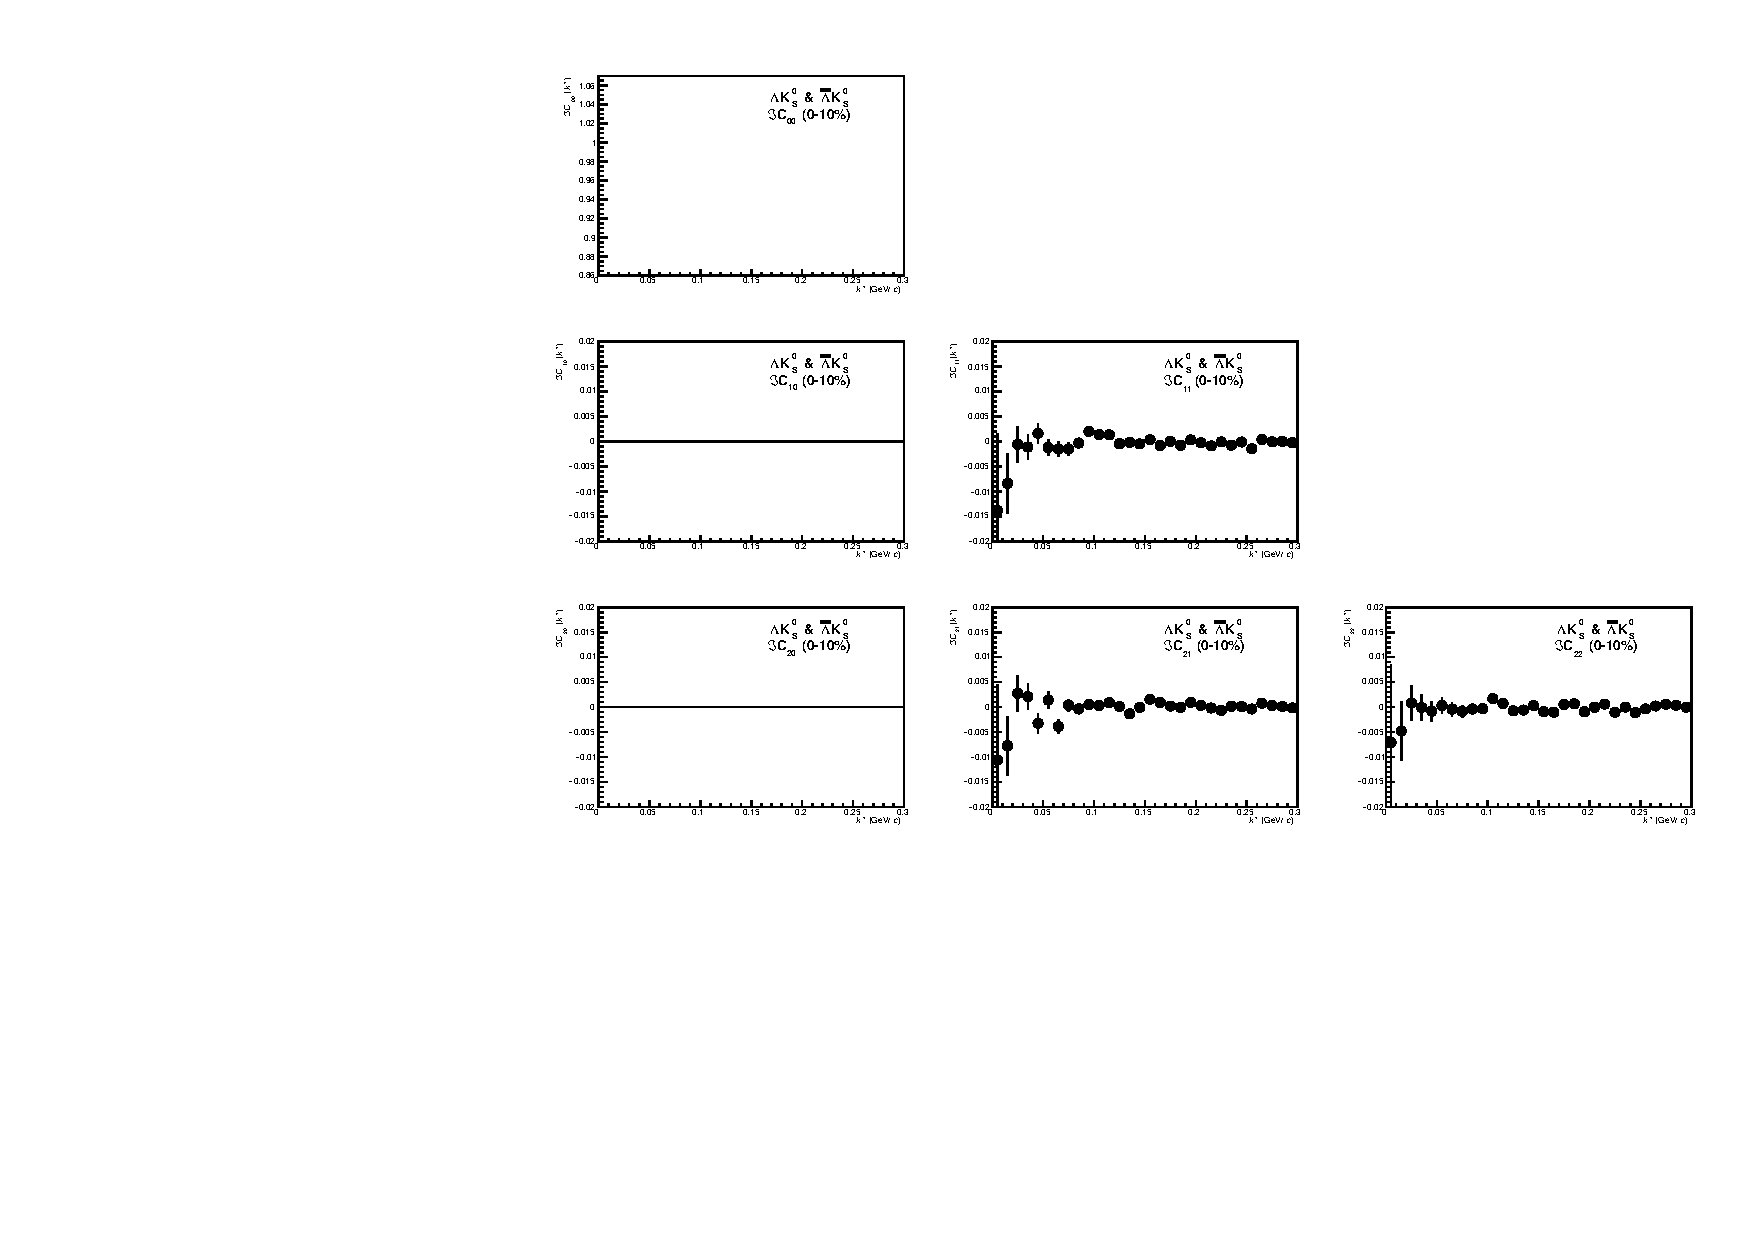
\includegraphics[width=0.50\linewidth]{\ResultsDirBase Results_cLamK0_20181205/SphericalHarmonics/LamK0/CanCfYlmImFirstSixComps_LamK0ALamK0_0010.pdf}}  
  %%----overall caption----
  \caption[Short Overall]{Long Overall}
  \label{fig:LamK0_FirstSixCYlm}
\end{figure}

\end{document}